\chapter{積分}%第4章

\begin{mysimplebox}{問1}
   $\int_{0}^{1+i}\Re(z)dz$($z=0$から$z=1+i$に至る線分に沿って)
\end{mysimplebox}
\paragraph{解}
この積分路では$z=x+ix$であり、$x$は0から1まで動くから
\begin{align*}
    \int_{0}^{1+i}\Re(z)dz
    &=\int_{0}^{1}xd(x+ix)
    =\int_{0}^{1}x(1+i)dx
    =(1+i)\left[\frac{x^2}{2}\right]_0^1
    =\frac{1+i}{2}
\end{align*}

\begin{mysimplebox}{問2}
    $\int_{-i}^{i}|z|dz$(円$|z|=1$の左半分に沿って)
 \end{mysimplebox}
 \paragraph{解}
 \begin{align*}
    \int_{-i}^{i}|z|dz
    &=\int_{\frac{3\pi}{2}}^{\frac{\pi}{2}}|e^{i\theta}|d(e^{i\theta})
    =\int_{\frac{3\pi}{2}}^{\frac{\pi}{2}}ie^{i\theta}d\theta
    =\left[e^{i\theta}\right]_{\frac{3\pi}{2}}^{\frac{\pi}{2}}
    =e^{\frac{\pi}{2}}-e^{\frac{3\pi}{2}}=i-(-i)=2i
\end{align*}

\begin{mysimplebox}{問3}
   $\int_{|z|=1}|z-1||dz|$(正の向き)
\end{mysimplebox}
\paragraph{解}
\begin{align*}
   \int_{|z|=1}|z-1||dz|
   &=\int_{0}^{2\pi}|e^{i\theta}-1||d(e^{i\theta})|
   =\int_{0}^{2\pi}|\cos \theta-1+i\sin \theta||ie^{i\theta}d\theta|\\
   &=\int_{0}^{2\pi}\sqrt{(\cos\theta-1)^2+\sin^2\theta}d\theta
   =\int_{0}^{2\pi}\sqrt{2(1-\cos\theta)}d\theta\\
   &=2\int_{0}^{2\pi}\sqrt{\sin^2\frac{\theta}{2}}d\theta
   =2\int_{0}^{2\pi}\left|\sin\frac{\theta}{2}\right|d\theta\\
   &=2\int_{0}^{2\pi}\sin\frac{\theta}{2}d\theta
   =2\left[-2\cos\frac{\theta}{2}\right]_0^{2\pi}\\
   &=-4(-1-1)=8
\end{align*}

\begin{mysimplebox}{問4}
   $\int_{|z|=1}\frac{e^z}{z^2}dz$(正の向き)
\end{mysimplebox}
\paragraph{解}
\begin{align*}
   \int_{|z|=1}\frac{e^z}{z^2}dz
   &=\int_{|z|=1}\frac{1}{z^2}\left(1+z+\frac{1}{2!}z^2+\dots\right)dz
   =\int_{|z|=1}\frac{1}{z}dz=2\pi i
\end{align*}

\begin{figure}[h]
   \centering
   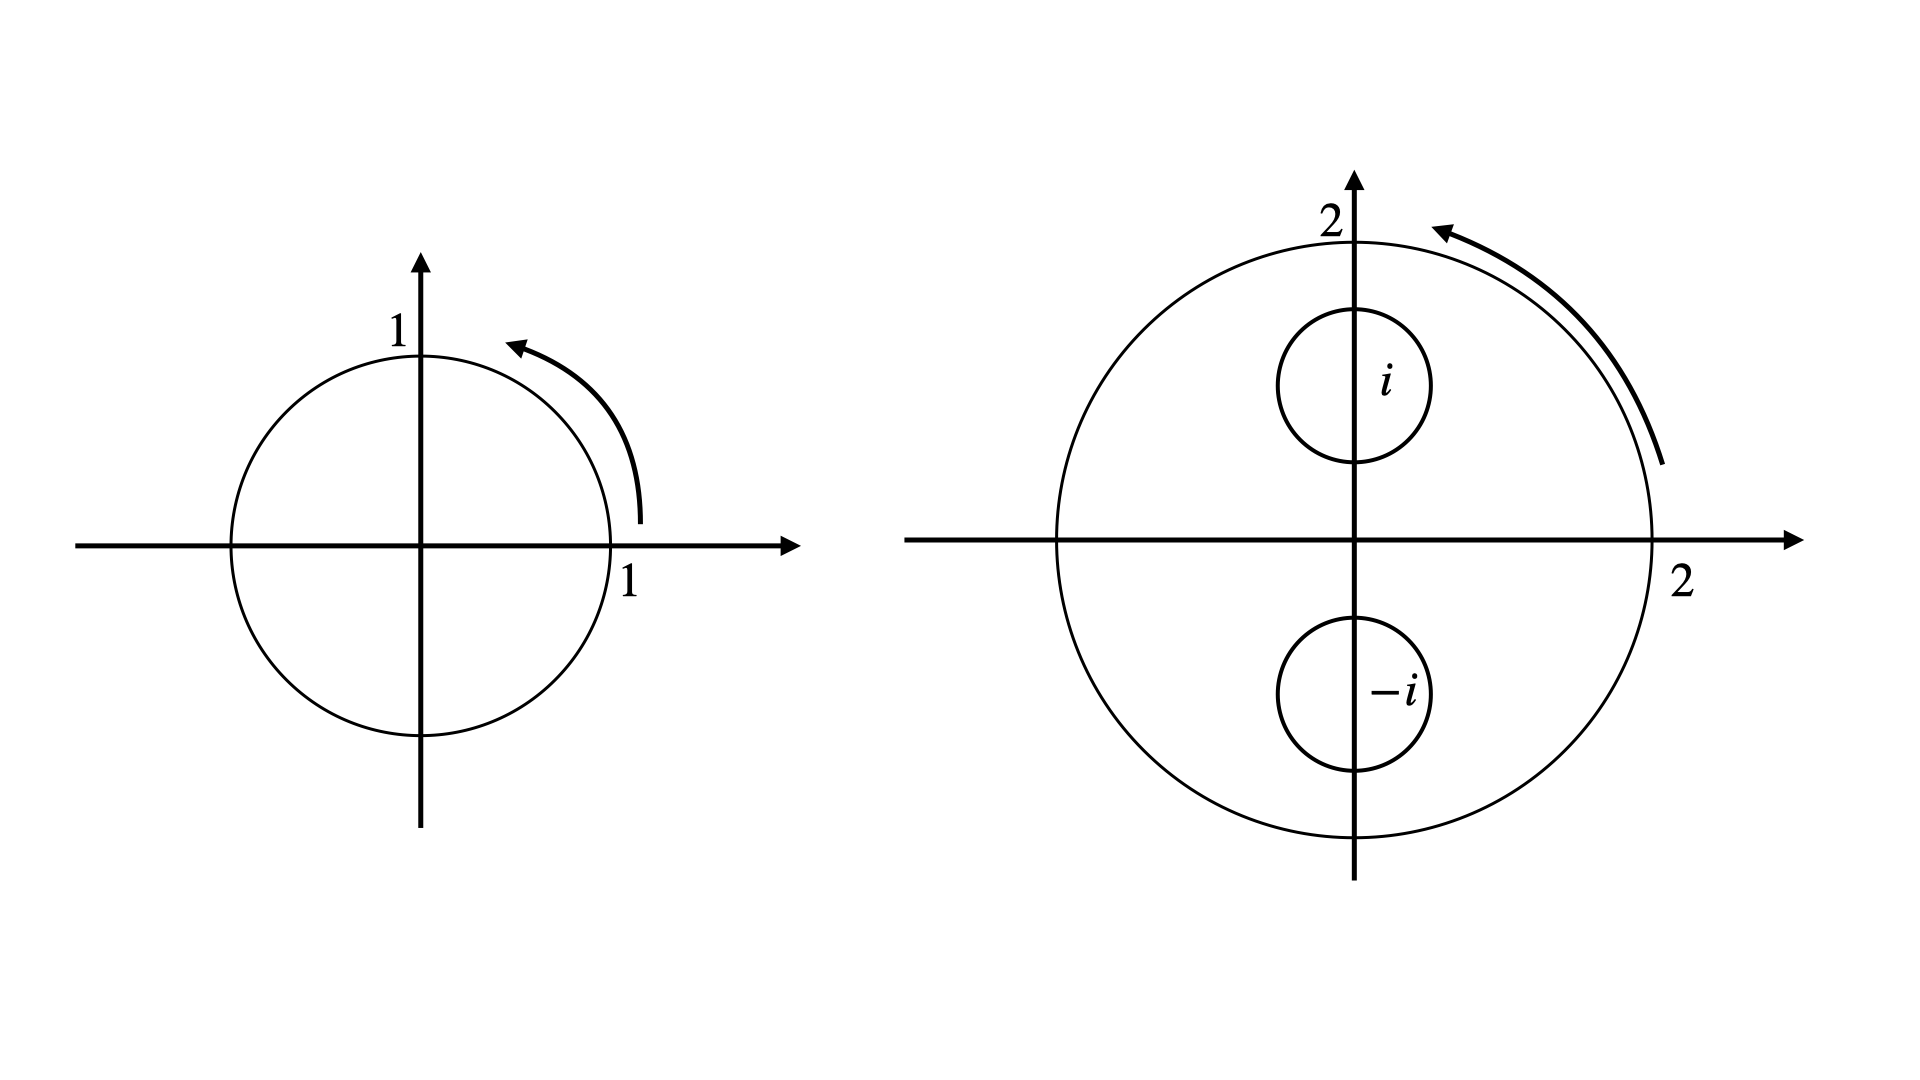
\includegraphics[width=10cm]{chap4_fig/chap4_fig001.png}
   \caption{積分路}
   \label{fig:chap4}
\end{figure}

\begin{mysimplebox}{問5}
   $\int_{|z|=2}\frac{dz}{1+z^2}$(正の向き)
\end{mysimplebox}
\paragraph{解}
\begin{align*}
   \int_{|z|=2}\frac{dz}{1+z^2}
   &=\int_{|z|=2}\frac{1}{2i}\left(\frac{1}{z-i}-\frac{1}{z+i}\right)dz
   =\frac{1}{2i}\left(\int_{|z|=2}\frac{dz}{z-i}-\int_{|z|=2}\frac{dz}{z+i}\right)\\
   &=\frac{1}{2i}(2\pi i-2\pi i)=0
\end{align*}

\begin{mysimplebox}{問6}
   $f(z)=\sum_{n=0}^{\infty}c_nz^n$の収束半径が$R(>0)$のとき
   \begin{align*}
      f(0)=\lim_{n\to\infty}\sum_{\nu=0}^{n}f(r\omega_n^\nu)\cdot n^{-1}\quad\left(0<r<R, \omega_n=\exp\left(\frac{2\pi i}{n}\right)\right)
   \end{align*}
   を示せ。
\end{mysimplebox}
\paragraph{証明}
$|r\omega_n^\nu|<R$であるから、$f(r\omega_n^\nu)$は収束する。

級数を次のように積分に変形できる。
\begin{align*}
   \frac{1}{n}\sum_{\nu=0}^{n}f(r\omega_n^\nu)
   &=\frac{1}{n}\sum_{\nu=0}^{n}f\left(r\exp\left(\frac{2\pi i\nu}{n}\right)\right)
   \overset{n\longrightarrow\infty}{\longrightarrow}
   \int_{0}^{1}f(r\exp(2\pi it))dt
\end{align*}

$f(z)$はべき級数であるから、項別積分可能である。
よって、
\begin{align*}
   \int_{0}^{1}f(r\exp(2\pi it))dt
   &=\int_{0}^{1}\sum_{n=0}^{\infty}c_nr^n\exp(2\pi int)dt
   =\sum_{n=0}^{\infty}c_nr^n\int_{0}^{1}\exp(2\pi int)dt\\
   &=c_0\int_{0}^{1}dt+\sum_{n=1}^{\infty}c_nr^n\int_{0}^{1}\exp(2\pi int)dt\\
   &=c_0+\sum_{n=1}^{\infty}c_nr^n\left[\frac{\exp(2\pi int)}{2\pi in}\right]_0^1\\
   &=c_0+\sum_{n=1}^{\infty}c_nr^n\frac{1}{2\pi in}\left\{\exp(2\pi in)-\exp(0)\right\}\\
   &=c_0=f(0)
\end{align*}
(証明終)

\begin{mysimplebox}{問7}
   \begin{align*}
      \int_{|z|=1}\left(z+\frac{1}{z}\right)^{2n}\frac{dz}{z}
   \end{align*}
   を求めることにより、
   \begin{align*}
      \int_{0}^{2\pi}\cos^{2n}\theta d\theta
      =2\pi\cdot\frac{1\cdot3\cdot5\cdot\dots\cdot(2n-1)}{2\cdot4\cdot6\cdot\dots\cdot2n}
   \end{align*}
   を示せ。
\end{mysimplebox}
\paragraph{証明}
$|z|=1$において$z=e^{i\theta}$であるから
\begin{align*}
   \int_{|z|=1}\left(z+\frac{1}{z}\right)^{2n}\frac{dz}{z}
   &=\int_{0}^{2\pi}\left(e^{i\theta}+\frac{1}{e^{i\theta}}\right)^{2n}\frac{de^{i\theta}}{e^{i\theta}}
   =\int_{0}^{2\pi}2^{2n}\cos^{2n}\theta\frac{ie^{i\theta}d\theta}{e^{i\theta}}\\
   &=2^{2n}i\int_{0}^{2\pi}\cos^{2n}\theta d\theta
\end{align*}

また、被積分函数を2項定理によって展開すると
\begin{align*}
   \int_{|z|=1}\left(z+\frac{1}{z}\right)^{2n}\frac{dz}{z}
   &=\int_{|z|=1}\sum_{k=0}^{2n}\binom{2n}{k}z^kz^{-(2n-k)}z^{-1}dz
   =\sum_{k=0}^{2n}\binom{2n}{k}\int_{|z|=1}z^{2k-2n-1}dz\\
   &=\binom{2n}{n}\int_{|z|=1}\frac{dz}{z}=2\pi i\binom{2n}{n}
\end{align*}

よって
\begin{align*}
   \int_{0}^{2\pi}\cos^{2n}\theta d\theta
   &=\frac{1}{2^{2n}i}2\pi i\binom{2n}{n}
   =2\pi\frac{1}{2^{2n}}\frac{(2n)!}{n!n!}\\
   &=2\pi\frac{(2n)!}{(2\cdot4\cdot6\cdots2n)^2}
   =2\pi\frac{1\cdot3\cdot5\dots(2n-1)}{2\cdot4\cdot6\cdots2n}
\end{align*}
(証明終)